%==============================================================================
\section{Results} \label{sec:resultados}
%==============================================================================

All figures come from a single identified run of the pipeline; trained weights, per-epoch histories, and per-fold metrics are preserved.
No subject was held out for testing, so all accuracy metrics are \textbf{validation} metrics, each subject being evaluated by the model of the fold in which it was not trained.
The three architectures completed the 100-epoch budget in all folds without divergence or severe overfitting, so neither the budget nor the family recipes were inadequate for any architecture.

%------------------------------------------------------------------------------
\subsection{Accuracy and statistical significance} \label{sec:res_acuracia}

Table~\ref{tab:comparacao_acuracia} reports both epoch-selection variants.
The best-epoch variant exceeds the final-epoch one for every architecture, as expected from selecting and reporting on the same partition.
In both variants and in all five folds the ranking is TransUNet $>$ U-Net $>$ \swinp{}, with no inversion.
Dice is below $2\,\mathrm{mIoU}/(1+\mathrm{mIoU})$ in every cell, as Jensen's inequality requires when both metrics are computed per class from the same predictions before averaging.
Fig.~\ref{fig:qualitativa_comparacao} shows predictions for samples chosen by quantitative criteria, each predicted with final-epoch weights by the model of the fold in which its subject was validated.

\begin{figure}[tbp]
\centering
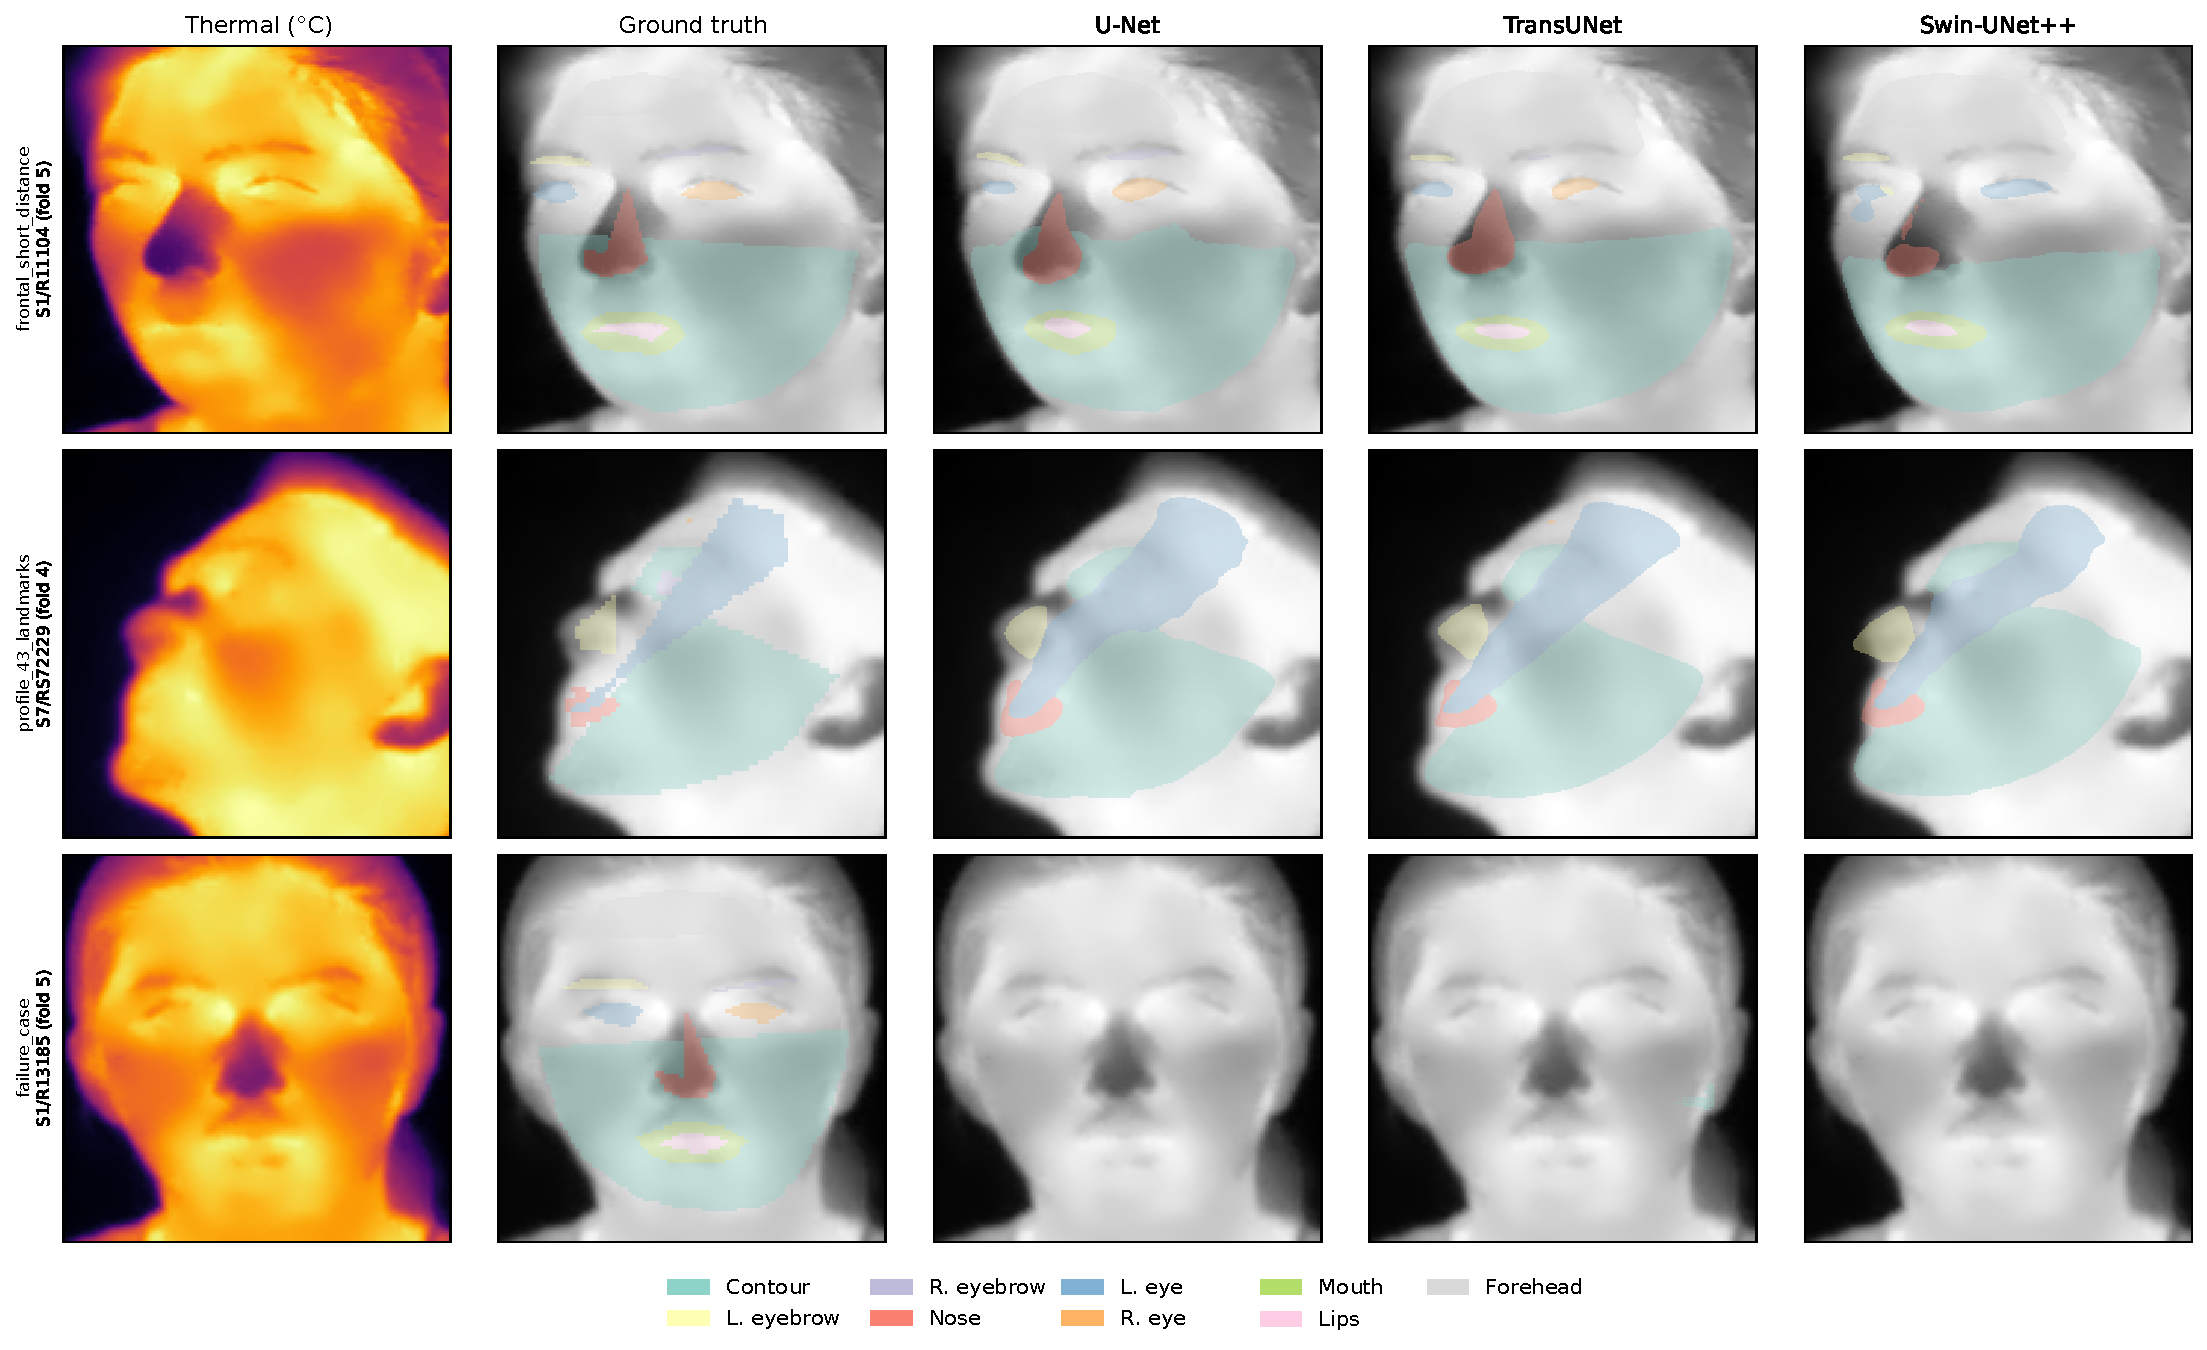
\includegraphics[width=\columnwidth]{img/resultados/fig_qualitativa-1.pdf}
\caption{Qualitative comparison. Columns: thermal image, derived reference, U-Net, TransUNet, \swint{}. Rows: closest annotated capture distance (frontal); median-performance profile view, showing the displaced ``left eye'' of Section~\ref{subsec:res_anomalia_lateral}; lowest-mIoU validation sample.}
\label{fig:qualitativa_comparacao}
\end{figure}

\begin{table}[tbp]
\centering
\caption{Accuracy (mean $\pm$ std.\ across the five folds)}
\label{tab:comparacao_acuracia}
\footnotesize
\setlength{\tabcolsep}{3pt}
\begin{tabular}{@{}lccc@{}}
\toprule
& \multicolumn{2}{c}{\textbf{Final epoch (primary)}} & \textbf{Best epoch} \\
\cmidrule(lr){2-3}\cmidrule(lr){4-4}
\textbf{Architecture} & \textbf{mIoU} & \textbf{Dice} & \textbf{mIoU} \\
\midrule
TransUNet & $\mathbf{0.4333 \pm 0.0491}$ & $\mathbf{0.5910}$ & $\mathbf{0.4471 \pm 0.0493}$ \\
U-Net & $0.4045 \pm 0.0527$ & $0.5599$ & $0.4191 \pm 0.0548$ \\
\swint{} & $0.3529 \pm 0.0430$ & $0.4978$ & $0.3743 \pm 0.0456$ \\
\bottomrule
\end{tabular}
\end{table}

Table~\ref{tab:comparacoes_pareadas} tests whether this ordering is distinguishable from experimental variability.
Under subject pairing, all three comparisons are significant, the bootstrap intervals exclude zero, and the Holm-adjusted $p$-value is $0.0059$ for each.
Fold pairing, with the same sign in 15 of 15 cases, cannot reach significance because its floor is $0.0625$.
Two of the three comparisons sit exactly at the floor of the $n=10$ test, so they are as significant as the design permits, and no more.
The subject-level view also reveals heterogeneity hidden by folds: TransUNet beats U-Net on 9 of 10 subjects, the exception being S6.

\begin{table}[tbp]
\centering
\caption{Paired comparisons of final-epoch mIoU}
\label{tab:comparacoes_pareadas}
\footnotesize
\setlength{\tabcolsep}{2.5pt}
\begin{tabular}{@{}lcccc@{}}
\toprule
\textbf{Comparison} & \textbf{$\Delta$mIoU} & \textbf{Wins} & \textbf{Wilcoxon $p$} & \textbf{95\% CI} \\
\midrule
\multicolumn{5}{@{}l}{\textit{Paired by subject ($n=10$), primary}} \\
TransUNet -- U-Net & $+0.0296$ & 9/10 & $\mathbf{0.0039}$ & $[0.016, 0.045]$ \\
U-Net -- \swint{} & $+0.0573$ & 10/10 & $\mathbf{0.0020}$ & $[0.036, 0.078]$ \\
TransUNet -- \swint{} & $+0.0868$ & 10/10 & $\mathbf{0.0020}$ & $[0.064, 0.110]$ \\
\midrule
\multicolumn{5}{@{}l}{\textit{Paired by fold ($n=5$), secondary}} \\
TransUNet -- U-Net & $+0.0288$ & 5/5 & $0.0625$ & $[0.019, 0.041]$ \\
U-Net -- \swint{} & $+0.0517$ & 5/5 & $0.0625$ & $[0.042, 0.064]$ \\
TransUNet -- \swint{} & $+0.0805$ & 5/5 & $0.0625$ & $[0.068, 0.093]$ \\
\bottomrule
\end{tabular}
\end{table}

%------------------------------------------------------------------------------
\subsection{Partition variability versus architecture effect} \label{subsec:res_variabilidade_particoes}

Averaging the three architectures within each fold measures the \textbf{difficulty of each partition}.
It ranges from $0.3444$ (fold 2) to $0.4439$ (fold 5), a spread of $\mathbf{0.0995}$, larger than the largest mean difference between architectures ($0.0868$, TransUNet vs.\ \swinp{}).
\textbf{Which subjects form the validation partition affects the measured mIoU more than the choice of architecture}, even between the best and the worst of the three.
A single train/test split would thus have yielded an estimate, and possibly a ranking, that depended on which subjects happened to be drawn.
A competing explanation is view composition: fold 2 has the largest share of profile views ($61.8\%$), whose masks are defective (Section~\ref{subsec:res_anomalia_lateral}).
The explanation does not survive stratification: restricted to frontal views, the hardest fold becomes fold 3 (U-Net $0.3788$ vs.\ $0.4109$ for fold 2), driven by subject S10, whose mIoU ($0.166$--$0.194$) is $4.15$ standard deviations below the other nine.
Fold ordering is explained by subject identity rather than by view composition.

%------------------------------------------------------------------------------
\subsection{Per-class performance and the lateral anomaly} \label{subsec:res_anomalia_lateral}

Table~\ref{tab:iou_por_classe} reports per-class IoU.
Large regions (background, lower contour, forehead) score highest in all architectures.
Across the nine foreground classes, mean IoU correlates with class area in the processed corpus (Spearman $\rho=+0.900$, $p=0.0009$), but only moderately and non-significantly with the area measured on frontal views, which are free of the defect described below ($\rho=+0.633$, $p=0.067$).
Area is thus a strong but not dominant factor; mask fidelity acts in the same direction.

\begin{table}[tbp]
\centering
\caption{Per-class IoU (best epoch, aggregated over folds)}
\label{tab:iou_por_classe}
\footnotesize
\setlength{\tabcolsep}{4pt}
\begin{tabular}{@{}lccc@{}}
\toprule
\textbf{Class} & \textbf{U-Net} & \textbf{TransUNet} & \textbf{\swint{}} \\
\midrule
Background & 0.8826 & 0.8976 & 0.8884 \\
Lower face contour & 0.7162 & 0.7623 & 0.7342 \\
Left eyebrow\textsuperscript{\textdagger} & 0.4176 & 0.4285 & 0.3288 \\
Right eyebrow\textsuperscript{\textdagger} & 0.3012 & 0.3213 & 0.1931 \\
Nose & 0.3771 & 0.4150 & 0.3359 \\
Left eye\textsuperscript{\textdagger} & 0.4958 & 0.5194 & 0.4788 \\
Right eye\textsuperscript{\textdagger} & 0.4190 & 0.4314 & 0.2325 \\
Mouth & 0.2891 & 0.3225 & 0.2983 \\
Lips & 0.2666 & 0.3104 & 0.2800 \\
Forehead & 0.4891 & 0.5133 & 0.4875 \\
\bottomrule
\multicolumn{4}{@{}l}{\textsuperscript{\textdagger}\,Lateralized classes affected by UB-27 and UB-30.}
\end{tabular}
\end{table}

\textbf{Observation.} Anatomically equivalent classes differ systematically by side: left exceeds right by $0.107$--$0.136$ IoU for eyebrows and $0.077$--$0.246$ for eyes.
Faces are roughly symmetric and no architecture favors one side of the image, so a gap that persists in all three architectures and all folds points to the \textbf{data}.
Two independent defects, both discovered from this pattern and missed by the pre-run audit, produce it.

\textbf{UB-27: landmark scheme resolved from the file header.}
The dataset annotates 73 landmarks on frontal views and 43 on profile views, but every annotation file declares 73 columns for all rows, and the code chose the scheme from the header.
Profile rows (50.0\% of the corpus) were therefore read with the 73-point mapping: mouth, lips, and forehead vanish from their reference, the right eye collapses to a vestigial vertex (19~px on average vs.\ 414~px on frontal views), and the left eye receives a large, displaced polygon (6{,}131~px vs.\ 429~px) built from points that belong to the lips and forehead (Fig.~\ref{fig:anomalia_lateral_visual}).
On profile views, the macro average thus covers about six classes instead of nine.

\textbf{UB-30: horizontal flip without label permutation.}
Since labels follow the observer's side, flipping moves a structure across the facial midline without swapping its label.
With flip probability $0.5$, ``left'' and ``right'' were assigned to both halves of the face, so for the four lateralized classes the label ceased to be a function of the image.
The fix, a label permutation performed atomically with the flip, is implemented and tested, but was not applied retroactively.

\begin{figure}[tbp]
\centering
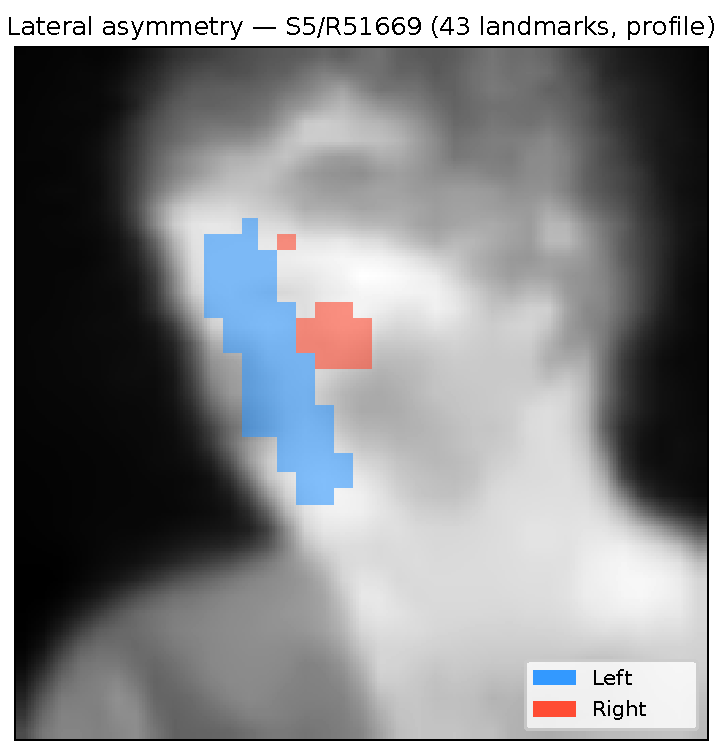
\includegraphics[width=0.48\columnwidth]{img/resultados/fig_anomalia_lateral-1.pdf}
\caption{Profile view with the derived lateral regions overlaid: the ``left eye'' (blue) is large and displaced; the ``right eye'' (red) is reduced to a vestige.}
\label{fig:anomalia_lateral_visual}
\end{figure}

\textbf{Robustness to the affected classes.}
Excluding the four lateralized classes (best-epoch aggregate), U-Net and \swinp{} differ by only $+0.0004$, whereas within those four classes U-Net leads by $+0.1001$: its whole advantage lies in classes whose labels were not a function of the image.
To test this, the 15 preserved final-epoch checkpoints were re-evaluated per subject, without retraining, on the macro of the five non-lateralized classes (Table~\ref{tab:comparacoes_5classes}).
TransUNet remains significantly ahead of both models even after Holm correction, while U-Net vs.\ \swinp{} becomes $+0.0040$ with 5/10 wins and $p=0.77$.
The robust answer to RQ1 is therefore the \textbf{partial ordering} TransUNet $>$ \{U-Net, \swinp{}\}.

\begin{table}[tbp]
\centering
\caption{Subject-paired comparisons on the five non-lateralized classes ($n=10$)}
\label{tab:comparacoes_5classes}
\footnotesize
\setlength{\tabcolsep}{3pt}
\begin{tabular}{@{}lcccc@{}}
\toprule
\textbf{Comparison} & \textbf{$\Delta$mIoU} & \textbf{Wins} & \textbf{Wilcoxon $p$} & \textbf{Holm} \\
\midrule
TransUNet -- U-Net & $+0.0437$ & 9/10 & $\mathbf{0.0039}$ & $\mathbf{0.0078}$ \\
U-Net -- \swint{} & $+0.0040$ & 5/10 & $0.7695$ & $0.7695$ \\
TransUNet -- \swint{} & $+0.0477$ & 10/10 & $\mathbf{0.0020}$ & $\mathbf{0.0059}$ \\
\bottomrule
\end{tabular}
\end{table}

\textbf{Ablation of UB-30.}
A second run, identical in seed, partitions, recipes, budget, and masks except for the flip fix, isolates UB-30.
On the five non-lateralized classes, \swinp{} rises from $0.4272$ to $0.4363$ and \textbf{overtakes} U-Net ($0.4266$), reversing the sign of their difference; TransUNet stays ahead in all folds.
On the four lateralized classes, however, \swinp{} drops from $0.3083$ to $0.2573$: under UB-27 the displaced polygon was consistently labeled ``left eye'' and hence learnable, whereas with permutation it alternates between labels.
Fixing one defect while leaving the other in place worsens the classes affected by both, so the two corrections must be applied together.
The corrected derivation (per-image scheme and visible side inferred from landmark geometry) has been verified on the full corpus but not yet used for retraining; absolute mIoU values are therefore a likely \textbf{lower bound}.

%------------------------------------------------------------------------------
\subsection{Computational efficiency} \label{sec:res_eficiencia}

Table~\ref{tab:custo_computacional} reports cost under the equalized conditions of Section~\ref{subsec:metricas_acuracia}.
\textbf{The speed ordering reverses the accuracy ordering}: \swinp{} is $1.6\times$ faster than U-Net and $2.3\times$ faster than TransUNet, uses the least inference memory, and trains $2.2\times$ faster per fold.
Although it has more parameters than U-Net ($40.9$~M vs.\ $31.0$~M), it uses about half the memory, because under a fixed batch peak memory is dominated by intermediate activations, which depend on the spatial resolutions kept through the network, not by weights.
Fig.~\ref{fig:fronteira_compromisso} summarizes the trade-off (RQ3): no architecture dominates; TransUNet maximizes accuracy at the highest latency and model size, \swinp{} minimizes cost at the lowest accuracy, and U-Net lies in between.

\begin{table}[tbp]
\centering
\caption{Computational cost (fixed batch of 4, GTX 1660 Ti)}
\label{tab:custo_computacional}
\footnotesize
\setlength{\tabcolsep}{2.5pt}
\begin{tabular}{@{}lcccccc@{}}
\toprule
\textbf{Arch.} & \textbf{ms/img} & \textbf{img/s} & \textbf{Peak (MB)} & \textbf{Size (MB)} & \textbf{Par.\,(M)} & \textbf{Train/fold} \\
\midrule
U-Net & 17.99 & 55.6 & 555.9 & 118.4 & 31.04 & 921.7 min \\
TransUNet & 25.53 & 39.2 & 591.7 & 403.2 & 105.71 & 908.7 min \\
\swint{} & \textbf{11.15} & \textbf{89.7} & \textbf{300.6} & 156.1 & 40.92 & \textbf{413.0} min \\
\bottomrule
\end{tabular}
\end{table}

\begin{figure}[tbp]
\centering
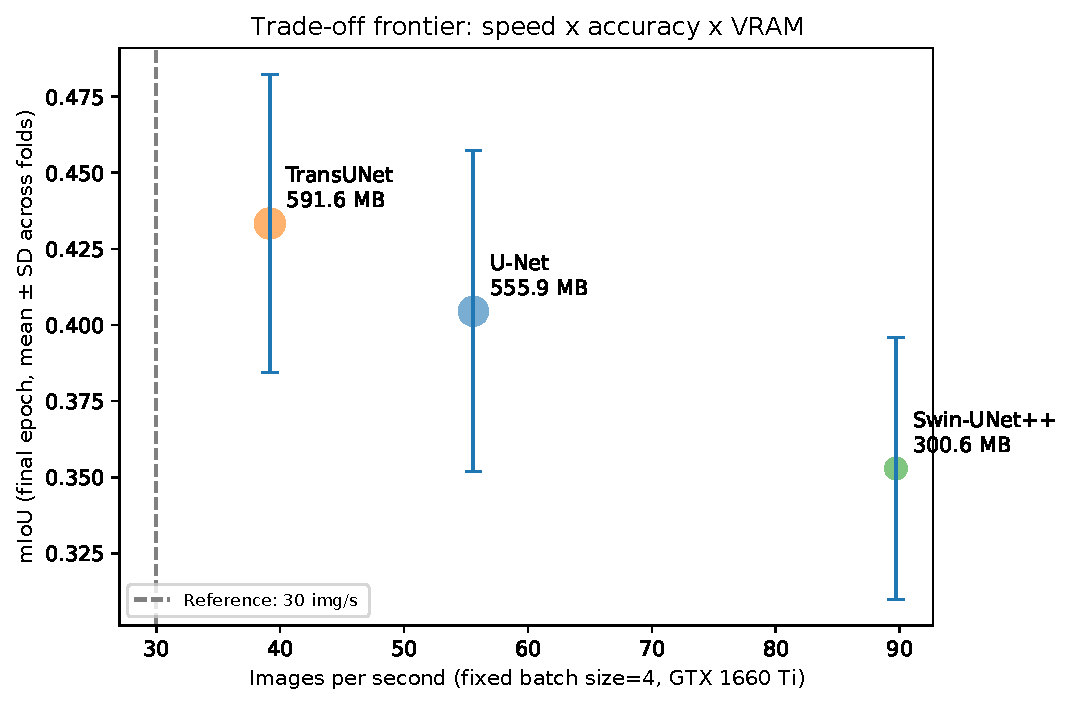
\includegraphics[width=0.92\columnwidth]{img/resultados/fig_pareto-1.pdf}
\caption{Accuracy--throughput trade-off. Error bars: $\pm1$ std.\ across folds; labels give peak inference memory (fixed batch of 4).}
\label{fig:fronteira_compromisso}
\end{figure}

\textbf{Two inversions of the memory ranking.}
Memory was measured incorrectly twice, and each error produced a different ranking.
The first measurement compared architectures under different batch sizes (UB-10) and ranked U-Net as the \textbf{most} memory-hungry.
The second fixed the batch but read the device-wide peak counter with all three models resident, so each was charged for the memory of those probed before it ($+30.9$, $+325.5$, and $+636.5$~MB).
It reported $586.7$, $917.1$, and $937.1$~MB, ranking U-Net as the \textbf{least} and \swinp{} as the most memory-hungry.
Only the isolated probe (UB-28) yields the values in Table~\ref{tab:custo_computacional}.
Latency had the same structural flaw, being originally measured under the per-architecture training batch sizes.

%------------------------------------------------------------------------------
\subsection{Capture distance} \label{sec:res_distancia}

Stratifying per-image mIoU by the quartiles of the annotated capture distance ($1.0$--$6.6$~m for $98.5\%$ of the corpus) shows no monotonic degradation.
All three architectures peak in the $2.8$--$4.0$~m range (e.g., TransUNet $0.457$ vs.\ $0.405$ at $1.0$--$1.8$~m), the architecture ranking holds in every range, and the peak persists when frontal and profile views are analyzed separately.
The within-range standard deviation ($0.12$--$0.16$) is two to three times the largest between-range difference ($0.05$).
Because faces are cropped and resized to $256\times256$, the apparent-size effect of distance is removed, and only blur and signal-to-noise effects remain; within the covered range, distance is not a dominant determinant of performance.
